\documentclass[11pt]{article}

\usepackage[margin=1.0in]{geometry}
%\linespread{1.5}
\usepackage{graphicx}
\usepackage{amsmath}
\usepackage{cite}

% definition of \customlabel, which is used to label supplementary figures and tables
\makeatletter
\newcommand{\customlabel}[2]{%
\protected@write \@auxout {}{\string \newlabel {#1}{{#2}{\thepage}{}{}{}}}}
\makeatother



\renewcommand{\bottomfraction}{.9}
\renewcommand{\topfraction}{.9}
\renewcommand{\textfraction}{0.1}
\renewcommand{\floatpagefraction}{.9}


\begin{document}
\title{\textbf{The relationship between dN/dS and ???}}
\author{Stephanie J. Spielman$^{1}$ and Claus O. Wilke$^{1}$}
\date{}

\maketitle
\noindent
Address:\\
$^1$Department of Integrative Biology, Center for Computational Biology and Bioinformatics, and Institute of Cellular and Molecular Biology.
The University of Texas at Austin, Austin, TX 78712, USA.\\

\bigskip
\noindent
$^*$Corresponding author\\
$\phantom{^*}$Email: ??????????\\

\bigskip
\noindent Keywords: mutation-selection-balance models, mechanistic codon models, $dN/dS$, equilibrium codon frequencies, natural selection, protein evolution, models of sequence evolution

\newpage
\begin{abstract}
Two models which investigate strength of selection in protein-coding sequences are mechanistic codon models and mutsel models. We have measures of dN/dS and amino acid/codon ``propensities", which correspond to equilibrium frequencies. Are they the same? Are they different? We don't know! But now we do. And they're the same. But there are some important consequences of this. For instance, codon bias. Also for instance, mech codon models seem ill-equipped to deal with asymmetric mutation rates and parameterizing them is really awkward.
  
\end{abstract}


\section*{Introduction}

Over the years, various methods have been used to calculate the strength of natural selection acting on protein-coding sequences. Traditionally, the focus has been on estimating the evolutionary rate ratio, $dN/dS$, the rate of nonsynonymous to synonymous substitution rates. This metric indicates how quickly a protein's constituent amino acids change, and is widely used to identify cases of positive, diversifying selection ($dN/dS > 1$) \cite{NielsenYang1998, Yangetal2000, KosakovskyPondFrost2005, Huelsenbecketal2006}. Following early counting methods for estimating $dN/dS$ (e.g. refs \cite{LWL85} and \cite{NG86}), mechanistic codon models, which assume an explicit Markov-process model of sequence evolution (see ref.~\cite{Anisimova2009} for a comprehensive review), have taken a leading role as the inference method of choice since their introduction in the 1990s \cite{GoldmanYang1994, MuseGaut1994, NielsenYang1998}. These models yield maximum likelihood estimates (MLEs) for the parameter $\omega$, which represents the quantity $dN/dS$, and have seen great success in the field of molecular evolution. 

A second class of models, known as mutation-selection-balance (MutSel) models, have emerged recently as a popular alternative to mechanistic codon models. The MutSel framework, couched firmly in population genetics theory, models the dynamic interplay between mutation and selection in a protein-coding sequence. MutSel models yield estimates of site-wise scaled selection coefficients, which indicate the extent to which natural selection favors, or disfavors, particular codons or amino acids at a given protein position. Although MutSel models were first introduced over 15 years ago \cite{HalpernBruno1998}, they have seen virtually no use due to their high computational expense. However, recently, several computationally tractable model implementations have emerged \cite{RodrigueLartillot2014,Tamurietal2014}, allowing for the first time the potential for widespread use. 


Although both mechanistic codon models and MutSel models describe the same fundamental process of protein-coding sequence evolution along a phylogeny, it is largely unknown how these two classes of models relate to one another. In particular, as these inference methods have been developed independently, it remains an open question whether or not parameter estimates from one model are comparable to those of the other model. Whether $dN/dS$ values have any correspondence with scaled selection coefficients remains an open question. Therefore, while certain rhetorical arguments may be made in favor of using one method over another, there is currently no formalized, concrete rationale to guide researchers in their methodological choices. 


Here, we show that $dN/dS$ can be precisely determined based on MutSel model parameters alone. Specifically, the estimates of fitness/mutation rates allows one to compute equilibrium frequencies. 
These equilibrium frequencies can then accurately estimate dN/dS.
Several important results 


Here, we formalize the relationship between mechanistic codon and MutSel models by examining the extent to which their focal parameters, $dN/dS$ and scaled selection coefficients, yield overlapping information about the evolutionary process. To this end, we derive a mathematical relationship these models' primary parameters from which one can infer $dN/dS$ values from selection coefficients alone. Using a simulation approach, we verify that $dN/dS$ values estimated using selection coefficients alone correspond precisely to $\omega$ MLEs inferred using standard mechanistic codon models. 

% MORE NEEDS TO BE WRITTEN HERE FOR SURE ONCE THE REST OF THE MS IS COMPLETE
(???)Further, we prove that, under conditions of symmetric mutation rates, this relationship holds only under regimes of purifying selection or neutral evolution ($dN/dS \leq 1$). This proof reveals that MutSel models are inherently unable to describe accurately protein evolution under a regime of positive diversifying selection, or when $dN/dS > 1$.

Moreover, our analyses incidentally have revealed certain biases inherent in the ML $\omega$ inference approach. (...)
 


\section*{Methods}

\subsection*{Sequence simulation}
We simulated protein-coding sequences as a continuous-time Markov
process \cite{Yang2006} according to the MutSel model proposed by \cite{HalpernBruno1998}. This model's instantaneous rate matrix $Q$ is given by 

\begin{equation}
Q_{ij} = \left\{ \begin{array}{rl}
              f_{ij}\mu_{ij}\kappa               &\mbox{single nucleotide transition} \\
              f_{ij}\mu_{ij}                          &\mbox{single nucleotide transversion} \\
              0                                           &\mbox{multiple nucleotide changes} \\             
         \end{array} \right.,
\end{equation}. Here, $\mu_{ij}$ is the nucleotide mutation rate and $f_{ij}$, the fixation probability from codon $i$ to $j$, is defined as \begin{equation}f_{ij} = ln\bigg{(}\frac{\pi_j\mu_{ij}}{\pi_i\mu_{ji}}\bigg{)}\bigg{/}\bigg{(}1 - \frac{\pi_i\mu_{ji}}{\pi_j\mu_{ij}}\bigg{)},\end{equation} where $\pi_i$ is the equilibrium frequency of codon $i$.



First, we simulated general data sets to show the theory.
To demonstrate the relationship between models, we simulated sequences with and without codon bias. For these simulations, we assumed a symmetric mutation matrix with $\mu_{xy} = 10^{-6}$ and $\kappa \sim \mathcal{U} (1,6)$. We simulated equilibrium codon frequencies $\pi_i$ according to a Boltzmann distribution, 
 \begin{equation}\label{eq:pi_i}
 \pi_i=\frac{e^{s_i}}{\sum_k e^{s_k}} ,
\end{equation} where the sum in the denominator runs over all 61 sense codons \cite{SellaHirsh2005}. The $s_i$ exponents were drawn from  $\mathcal{N}(0,\sigma^2)$, where $\sigma^2 \sim \mathcal{U}(0,4)$. Note that, in the presence of a symmetric mutation matrix, equation \eqref{eq:pi_i} suffices to determine the precise codon equilibrium frequencies \cite{SellaHirsh2005}. $\sigma^2$ effectively represents the strength of natural selection; larger values of $\sigma^2$ will correspond to greater equilibrium frequency differences among codons, and thus more selective pressure. 

For simulations which did not consider codon bias, we assigned all synonymous codons the same value $s_i$, thus leading to equal steady-state frequencies among synonymous codons. For simulations which incorporated codon bias, we first derived the codon frequencies expected in the absence of bias, and then converted them as follows. Assume that the equilibrium frequency of a codon in a given amino acid family, in the absence of bias, is $P$, and $k$ is the size of the codon family. We randomly selected one of these codons to be the preferred, and assigned it a frequency of $\pi_{preferred} = P(1 + \lambda(k-1))$, and all remaining codons were assigned the frequency $\pi_{non-preferred} = P(1 - \lambda)$. Here, $\lambda \sim \mathcal{U}(0,1)$ represents the extent of codon bias. When $\lambda = 0$, all synonymous codons have the same frequency, and when $\lambda = 1$, only one codon has a non-zero frequency. This codon bias model further ensures that each amino acid's equilibrium frequency remains unchanged, while partitioning this value differently among its codons.


Second, we used real data! We used real amino acid preference and nucleotide mutation rate data. For these sets, we used Jesse's amino acid preferences and Jesse's mu as well as yeast mu. For these cases, as real, asymmetric mutation rates were used, we had to determine the codon equilibrium frequencies $\pi_i$ under detailed balance, such that they satisfied the relationship $\pi_i\mu_ij = \pi_j\mu_ji$. 



We define the null codon frequencies as the those which are expected in the absence of of amino-acid level selection but which would be produced by mutation rates alone. We computed these null frequencies in the way as the equilibrium codon frequencies, except we assigned all amino acids the same preference value of 0.05, thus eliminating any amino-acid level fitness differences.


We simulated protein-coding sequences along a 4-taxon phylogeny, beginning with a root sequence selected using steady-state codon frequencies.Unless otherwise stated, all simulated alignments contained 500,000 codon positions. A single evolutionary model was applied to all positions in the simulated sequences. While this lack of site-wise heterogeneity is unrealistic for real sequence evolution, it allows us to verify our derived relationship between equilibrium codon frequencies and $dN/dS$ with a sufficiently sized data set.



\subsection*{$dN/dS$ Inference}
We calculated a global $dN/dS$ for each alignment using the mathematical framework outlined in \eqref{eq:pi_i}--\eqref{eq:dS} as well using standard maximum likelihood methods. Specifically, inferred $dN/dS$ using the M0 mechanistic codon model \cite{Yangetal2000}, as implemented in the HyPhy batch language \cite{KosakovskyPondetal2005}. The M0 models uses the GY94 instantaneous rate matrix \cite{GoldmanYang1994,NielsenYang1998}, which includes the primary parameters $\omega$, $\kappa$, and equilibrium codon frequencies. As different $\kappa$ and equilibrium codon frequency parameterizations can change $\omega$ estimates \cite{YN00, Yang2006, ZhangYu2006}, we inferred $\omega$ under a variety of model parameterizations, including three $\kappa$ parameterizations ($\kappa$ fixed to 1, $\kappa$ as a free parameter, and $\kappa$ fixed to its true value), and four codon frequency specifications (Fequal (all sense codons have an equilibrium frequency of 1/61),  F3x4 codon frequencies \cite{MuseGaut1994}, CF3x4 codon frequencies \cite{Pond2010} and F61, or empirical codon freqencies \cite{GoldmanYang1994}), ultimately resulting in 12 $\omega$ MLEs per simulated alignment. Note that we additionally verified that the system was evolving under a state-state process by verifying that the true, simulated codon frequencies were the same as the empirical codon frequencies calculated from the simulated alignment. All code used is freely available at \textbf{github}. 



\section*{Results}


\section*{Mathematical relationship between $dN/dS$ and equilibrium codon frequencies}


We describe here how to calculate $dN/dS$ from steady-state codon frequencies. The fixation probability for a mutation from codon $i$ to codon $j$ is \cite{HalpernBruno1998,SellaHirsh2005}
\begin{equation}\label{eq:f_ij}
 f_{ij} = \frac{1-(\pi_i/\pi_j)^{1/N_e}}{1-\pi_i/\pi_j}
  \approx \frac{1}{N_e} \frac{\ln \pi_j - \ln \pi_i}{1-\pi_i/\pi_j}\,,
\end{equation}
where $N_e$ is the effective population size. Using this framework, we can calculate an evolutionary rate by summing over all substitution probabilities weighted by the frequency of the originating codon. Further, we can establish specific expressions for nonsynonymous and synonymous evolutionary rates, and then divide them in order to obtain a value for the evolutionary rate ratio $dN/dS$.

To begin, we can write the nonsynonymous rate $K_\text{N}$ as 
\begin{equation}\label{eq:KN}
  K_\text{N} = N_e \sum_i \sum_{j \in {\cal N}_i} \pi_i  f_{ij}\mu_{ij}\,,
\end{equation}
where ${\cal N}_i$ is the set of codons that are nonsynonymous to codon $i$ and differ from it by one nucleotide. To normalize $K_\text{N}$, we divide it by the number of nonsynonymous sites, which we calculate according to the mutational opportunity definition of a site \cite{GoldmanYang1994, Yang2006} as 
\begin{equation}\label{eq:LN}
  L_\text{N} = \sum_i \sum_{j \in {\cal N}_i} \pi_i \mu_{ij}\,, 
\end{equation} and thus we find that 
\begin{equation}\label{eq:dN}
  dN = \frac{K_\text{N}}{L_\text{N}}=\frac{ N_e \sum_i \sum_{j \in {\cal N}_i} \pi_i f_{ij} \mu_{ij} } {\sum_i \sum_{j \in {\cal N}_i} \pi_i \mu_{ij} }\,.
\end{equation}

Similarly, for $dS$, the synonymous evolutionary rate $K_\text{S}$ per synonymous site $L_\text{S}$, we find
\begin{equation}\label{eq:dS}
  dS = \frac{K_\text{S}}{L_\text{S}}=\frac{ N_e \sum_i \sum_{j \in {\cal S}_i} \pi_i f_{ij} \mu_{ij} } {\sum_i \sum_{j \in {\cal S}_i} \pi_i \mu_{ij} }\,,
\end{equation}
where ${\cal S}_i$ is the set of codons that are synonymous to codon $i$ and differ from it by one nucleotide substitution. The quantities $K_\text{S}$ and $L_\text{S}$ are defined as in Eqs.~\eqref{eq:KN} and \eqref{eq:LN} but summing over $j\in {\cal S}_i$ instead of $j\in {\cal N}_i$.

Equations \eqref{eq:f_ij}--\eqref{eq:dS} establish a connection between the equilibrium codon frequencies and the evolutionary rate ratio $dN/dS$. Moreover, we note that, if we assume that all synonymous codons have equal fitness (e.g. synonymous mutations are neutral), the synonymous fixation rate $f_{ij}= 1/N_e$ \cite{CrowKimura1970}. Under this circumstance, the value for $dS$ reduces to 1.

\subsection*{$dN/dS$ can be accurately predicted from equilibrium codon frequencies}

To validate the mathematical relationship between steady-state codon frequencies and $dN/dS$ described in equations \eqref{eq:f_ij}--\eqref{eq:dS}, we simulated protein-coding sequences along a 4-taxon phylogeny according to a mutation-selection model framework \cite{HalpernBruno1998,SellaHirsh2005}. We simulated 100 alignments in which synonymous codons had equal frequencies, and 100 alignments with codon bias, e.g. where the equilibrium frequencies differed among synonymous codons (see Methods for details). All simulations assumed an underlying symmetric nucleotide rate matrix, with the transition-tranversion bias ratio $\kappa \sim \mathcal{U}(1,6)$. For each alignment, we calculated $dN/dS$ using equations \eqref{eq:f_ij}--\eqref{eq:dS} as well as using the M0 mechanistic codon model \cite{NielsenYang1998}, as implemented in the HyPhy batch language \cite{KosakovskyPondetal2005}.

The relationship between $dN/dS$ measurements is shown in Figure~\ref{reg_conv}A (for simulations with no codon bias) and Figure~\ref{reg_conv}B (for simulations with codon bias). It is clear that $dN/dS$ values derived using codon frequencies agree nearly perfectly with those inferred using standard maximum likelihood methods, and frequency differences among synonymous codons do not influence this robust relationship. Additionally, in Figure~\ref{reg_conv}C, we demonstrate convergence of $dN/dS$ estimates as the size of the data set, represented by simulated alignment length, increases. Taken together, these results demonstrate that MutSel model parameters fully encapsulate information regarding $dN/dS$, and that the results from MutSel and mechanistic codon models are in complete agreement.

We can additionally examine the extent to which $dN/dS$ relates to the strength of natural selection. As we employed a symmetric mutation matrix in these simulations, the codon equilibrium frequencies correspond precisely to codon fitness values \cite{SellaHirsh2005,deVladar2011}. Therefore, the distribution of equilibrium codon frequencies in fact represents the strength of purifying selection; when selection is strong, relatively fewer codons will be selectively tolerated, and thus the frequency distribution will be narrow. To examine the relationship between $dN/dS$ and selective strength, we computed the Shannon entropy \begin{equation}
        H = - \sum_i\pi_{i}\ln \pi_{i},
\end{equation}} where the sum runs over all 61 sense codons, for each set of equilibrium codon frequencies. Here, lower entropies correspond to more stringent purifying selection. Note that the maximum value of $H=4.11$ is achieved when all codons have an equal frequency of $1/61$. Figure~\ref{entropy_dnds} demonstrates that $dN/dS$ scales excellently with codon entropy; as entropy increases, $dN/dS$ similarly increases, properly reflecting the decrease in selection pressure. Moreover, while this trend holds both with and without the presence of synonymous codon fitness differences, the relationship between codon entropy and $dN/dS$ is stronger for simulations without codon bias (Figure~\ref{entropy_dnds}A, $r^2 = 0.901$) than with codon bias (Figure~\ref{entropy_dnds}B, $r^2 = 0.493$). This difference emerges from the fact that simulations with codon bias featured frequency, and hence fitness, differences among synonymous codons, obscuring the overarching fitness differences among amino acids.

Figure~\ref{entropy_dnds}A also shows that, as codon entropy approaches its maximum value of 4.11, $dN/dS$ approaches, but never exceeds, the value of 1. In fact, in \textbf{SI proof}, we prove that, when synonymous codons have equal equilibrium frequencies, $dN/dS$ is necessarily always less than or equal to 1. This restriction does not, however, hold in the face of codon bias, which can readily yield $dN/dS$ values greater than 1 (Figures \ref{reg_conv}B and \ref{entropy_dnds}B), even though the protein sequence is evolving according to a steady-state process. We discuss the implications of these findings in depth in \textit{Discussion}.


\subsection*{Issues with interpretations of $dN/dS$ values}

$dN/dS$ is used as a hallmark identifier for the three natural selection paradigms of purifying selection ($dN/dS < 1$), neutral evolution ($dN/dS = 1$), and finally positive selection ($dN/dS > 1$). Our analysis revealed that this classical $dN/dS = 1$ threshold might not be universally applicable. Indeed, all simulations presented here relied on the protein evolving under a steady-state process, or in other words, along a static fitness landscape. In a system where selective pressures remain constant along the phylogeny time, we expect purifying selection to dominate, and thus we should to recover only $dN/dS$ values less than 1. However, this was demonstrably not the case in several simulations which incorporated synonymous codon frequency, or fitness, differences (Figures~\ref{reg_conv}B and \ref{entropy_dnds}B). While simulations without codon bias all yielded $dN/dS < 1$, many simulations that incorporated codon bias featured $dN/dS$ values well above 1, with a maximum $dN/dS = 1.82$. In fact, we prove in \textbf{SI proof} that, under general conditions of a symmetric mutation and equal synonymous codon frequencies, $dN/dS$ is necessarily always less than or equal to 1. This proof, however, does not extend to cases of synonymous fitness differences, in spite of the steady-state evolutionary process. 

Moreover, we have found that that classical definition of neutral evolution as $dN/dS = 1$ may not be apt. Under neutral evolution, we expect that natural selection has no preference for specific amino acids or codons, but rather tolerates them all equally well. We can easily calculate $dN/dS$ under these conditions by assigning all amino acids the same steady-state frequency, again under a symmetric mutation matrix, of 0.05, and then distributing these frequencies evenly among synonymous codons. In other words, if an amino acid has four codons, each of those codons would have an equilibrium frequency of $0.05/4 = 0.0125$. Strikingly, the resulting $dN/dS$ value for this scenario is not 1, but instead equals 0.9125. Note that $dN/dS$ here is marginally affected by mutation rates (e.g., the inclusion of $\kappa$), but only by, at most, 1.4\%. Alternatively, if we instead compute $dN/dS$ based on equal \textit{codon}, rather than amino acid, equilibrium frequencies, $dN/dS$ does indeed come out to 1. Even though this scenario features neutral evolution's canonical $dN/dS=1$ signature, it does not biological correspond to neutral evolution; due to the redundancy of the genetic code, equal codon frequencies will necessarily result in unequal amino acid frequencies.

Thus, even under simple mathematical conditions, the codon-based metric of $dN/dS$ does not always accurately reflect amino-acid level processes. In other words, $dN/dS$ effectively can capture selective effects acting on codons, but not on amino acids. We discuss these findings more in depth in \textit{Discussion}.


\subsection*{Use of realistic data is also ok.}

Results reported in the previous subsections were obtained from fully-simulated equilibrium codon frequencies, along with a symmetric mutation matrix. The latter assumption of a symmetric mutation process (e.g. where $\mu_{xy} = \mu_{yx}$) may not be entirely realistic. Indeed, mutational bias, typically $C/G \rightarrow T/A$, is known to contribute to biased nucleotide compositions \cite{Hernandez2007,HershbergPetrov2010,Zhu2014,Acevedo2014}. Therefore, we performed additional simulations which made use of realistic amino acid fitness and nucleotide mutation parameters.
 In particular, we used influenza nucleoprotein (NP) site-specific amino acid preference values, given by Bloom \cite{Bloom2014a}. These data consisted of experimentally-determined fitness values for each individual amino acid across all 498 sites in NP, yielding 498 site-wise amino acid propensity distributions. We combined these experimental fitness parameters with three sets of experimentally determined mutation rates, either for NP \cite{Bloom2014a}, yeast \cite{Zhu2014}, or polio virus \cite{Acevedo2014}. Importantly, all of these mutation matrices are asymmetric, but feature differing degrees of asymmetry, with NP mutation rates being the most symmetric and polio mutation rates the most asymmetric. For each of the 498 amino acid fitness distributions, we calculated steady-state codon frequencies $\pi_i$ under detailed balance, such that the relationships $\pi_i\mu_{ij} = \pi_j\mu_{ji}$ and $\sum\pi_i = 1$, where the sum runs across all 61 sense codons, were satisfied, as described in \cite{Bloom2014a,Bloom2014b}.

\textbf{note to self - possible clarity problems with saying equilibrium frequencies. something it's a model parameter, sometimes it's the true freqs. be careful.}
We simulated 4-taxa alignments using these resulting equilibrium frequencies, and inferred $\omega$ using the M0 mechanistic codon model, as described in Methods. Here, we inferred $\omega$ according to eight different codon frequency parameterizations, as follows. First, we inferred $\omega$ using the Fequal \cite{Yang2006} parameterization, which assigns equal codon frequencies of $1/61$ each. Second, we inferred $\omega$ by specifying codon frequencies which would arise strictly from mutational processes in the absence of natural selection. We term this frequency parameterization ``Fnull." Finally, we used the common frequency estimators F3x4 \cite{MuseGaut1994}, CF3x4 \cite{Pond2010}, and F61 \cite{GoldmanYang1994}. In particular, we specified, for each of these three parameterizations frequency estimator, ``site" and ``global" codon frequencies. The site frequencies, denoted F3x4\_S, CF3x4\_S, and F61\_S, were computed individually for each set of true codon equilibrium frequencies. The global frequencies, denoted as F3x4\_G, CF3x4\_G and F61\_G, were calculated by pooling all 498 site-wise true codon frequencies to derive, effectively, average protein-wide values for equilibrium codon frequencies. These global parameterizations mirror the approach taken in real analyses, which consider the model's codon frequency parameters as protein-wide rather than site-specific. 

Resulting $\omega$ inferences correlate extremely well with $dN/dS$ values, but, as expected, the strengths of these correlations differ among codon frequency model parameterizations. Figure~\ref{nyp_bias_corr} shows the resulting relationships between $dN/dS$ values and $\omega$ MLEs for each set of mutation rates (NP, yeast and polio), across model frequency parameterizations. Figure~\ref{nyp_bias_corr}A displays the bias, or systematic deviation from a 1:1 relationship, between $dN/dS$ and $\omega$, and Figure~\ref{nyp_bias_corr}B displays the Pearson correlation between $dN/dS$ and $\omega$.

Overall, global frequency parameterizations feature the least amount of bias, and of the global estimators, Fequal results show the most noise. As expected, the Fnull generally outperforms all other frequency parameterizations in that is has very little bias and very little noise. F3x4\_G, CF3x4\_G, and F61\_G all perform roughly the same, although F61\_G performs relatively poorly for the NP mutation rate simulations. Alternatively, all site-wise codon frequency parameterizations produce inaccurate $\omega$ MLEs, exhibiting substantial bias and strong, negative correlations, and F61\_S performs even worse than do F3x4\_S and CF3x4\_S. 

The poor performance of site-wise frequency estimators can be readily explained by recognizing that that the rationale for including codon frequency parameters in mechanistic codon models is to account for unequal nucleotide frequencies specifically caused by mutational but not selective forces \cite{YN00, Yang2006}. Thus, codon frequency parameters should take on values of what the equilibrium codon frequencies would be \textit{in the absence of natural selection}. Using site-wise frequency parameters, therefore, effectively represents a model misspecification, as the true codon equilibrium frequencies are shaped by both mutation and natural selection. When site-based frequency parameterizations are used, these frequency parameters actually incorporate information about the strength of natural selection, rather than allowing the $\omega$ parameter alone to capture selective effects. Thus, the $\omega$ parameter no longer actually represented the evolutionary rate ratio $dN/dS$, and the strength of natural selection was improperly inferred as quite weak. Indeed, this misspecification led to dramatically elevated $\omega$ MLEs; for for example, when inferred using F61\_S, $\omega$ MLEs were as high as 10.18, 9.14, and and 13.67 for NP, yeast, and polio mutation rates, respectively.  These results emphasize that it is crucial to parameterize mechanistic codon models properly. Indeed, their primary parameter $\omega$ will only truly represent $dN/dS$ when all other parameters are properly specified. 

%We can calculate an asymmetry ``factor" for each set of mutation rates by finding the average value of $\mu_{xy}/\mu_{yx}$, where we further ensure that this quantity is greater than 1 for mathematical goodness. The asymmetry factor for NP, yeast, and polio mutation rates are 1.029, 1.655, and 4.45, respectively. 

It's also really nice to see that bias for the NP is the highest. This is because np had the least amount of asymmetry in its mutation rates, and thus the frequencies more closely represent the actual fitnesses. Thus, all selection info is inside the F61, effectively a total model misspecification.



While null performs the best, the $\omega$ -$dN/dS$ show a marked decrease as asymmetry increases. This suggests that the codon frequency parameters do not entirely capture what they are meant to. Remember, the only way for $\omega$ to equal $dN/dS$ is if the rest of the parameters are correct. Otherwise, it represents some quantity $\omega$. 

The asymmetry-induced trends are also apparent in the relationship between codon entropy and $dN/dS$. Recall, when mutation rates are symmetric, equilibrium codon frequencies correspond precisely to codon fitness values \cite{SellaHirsh2005}, and thus selective strength. The relationship between entropy and $dN/dS$ gets noisier as mutation rates become more asymmetric. This result perfectly reflects the dual influences of selection and mutation on equilibrium frequencies. The more that uneven mutation rates influence frequencies, the more noise there is. 


\subsection*{Discussion}

% may be useful to mention that many frameworks for dnds inference have been put forth over the years, and they are known to give conflicting results. Our approach to dnds inference is markedly different from these approaches, as it rests on population genetics principles rather than merely counting sites.
% our derivation yields the same results as does the standard, most-assumed-correct mech codon model. But it is clear that it is difficult to parameterize these models properly, especially given issues with codon frequencies not exactly doing what you what them to do, and likely being biased by sequence length. 
% this approach does, however make the assumption that there are indeed equilibrium codon frequencies that may be used. If a protein is evolving according to non-equilibrium processes, then there are no eq codon freqs, so this method is moot.
% previous efforts comparing among dnds calc methods all suffer because they all basically follow the same approach, except for how to deal with sites. This is really the difference among them. Here, this problem is basically removed.



The oldest and most-widely used method to infer selection pressure in protein-coding genes calculates calculates the ratio of non-synonymous ($dN$) to synonymous ($dS$) substitution rates $dN/dS$ to identify sites that experience negative selection ($dN/dS<1$), sites that evolve neutrally ($dN/dS\approx1$), and sites that experience positive diversifying selection ($dN/dS>1$). By contrast, MutSel models equilibrium amino acid and/or codon steady state frequencies and selection coefficients \cite{HalpernBruno1998,NielsenYang2008,Rodrigueetal2010,Tamurietal2012,Tamurietal2014}, for codons \cite{YangNielsen2008}, or for both. Thus, while mechanistic codon models describe the how quickly a protein's constituent amino acids change, MutSel models calculate the strength of natural selection operating on the specific amino-acid changes.  

Until now, however, it has been an open question how these two modeling frameworks relate to one another. Some have argued that MutSel models, given their firm grounding in population genetics theory and attention to site-specific amino acid fitness differences, offer a more fine-grained approach to studying protein evolution than do mechanistic codon models \cite{HalpernBruno1998,Rodrigueetal2010}. Recent phylogenetic studies have also demonstrated that evolutionary models which explicitly consider amino acid fitness values offer dramatic improvements over other models, including mechanistic codon models, suggesting that MutSel models may more aptly represent the process of coding-sequence evolution \cite{Bloom2014a, Bloom2014b}. 

Here, we have derived a formal mathematical relationship between the quantities $dN/dS$ and scaled codon selection coefficients, the primary parameters of mechanistic codon and MutSel models, respectively. Through a simulation approach, we find that these two models are in full agreement, and that the value for $dN/dS$ can be precisely calculated from selection coefficients alone. Furthermore, this mathematical equivalency between selection coefficients and $dN/dS$ values is robust to fitness differences among synonymous codons. However, it is important to note that our implementation of codon bias explicitly assumed that frequency differences among synonymous codons resulted from fitness differences alone. In other words, the sole source of codon bias in our simulations was selection, not mutation. This implementation might not be entirely biologically realistic, as both mutational and selective forces likely contribute to codon bias in real genomes \cite{Blumer1991, Duret2002, HershbergPetrov2008, PlotkinKudla2010}. However, the key finding that we present is that fitness differences among synonymous codons do not affect the robust mathematical equivalency between scaled selection coefficients and $dN/dS$. 


Our results rest on the key assumptions that the protein sequence is evolving under steady-state, or equilibrium, conditions, and the nucleotide mutation rates are symmetric (e.g. $\mu_{xy} = \mu_{yx}$). The first assumption recapitulates the population genetics theory behind MutSel models, which assume that selection coefficients remain constant over the phylogeny, and therefore the protein is evolving along a static fitness landscape \cite{HalpernBruno1998,Rodrigueetal2010,Tamurietal2012}. While the latter assumption of symmetric mutation rates may not be biologically realistic \textbf{cite papers which show asym mu}, it allowed us to investigate the mathematical relationship between $dN/dS$ and selection coefficients under broad conditions. In particular, we have proven that, when synonymous codons have equal fitness and mutation rates are symmetric, $dN/dS$ will always be less than 1. However, when synonymous codons were allowed to have different selection coefficients, $dN/dS$ can easily be greater than 1, and indeed frequently was (Figures \ref{reg_conv}B and \ref{stddev_dnds}B). In fact, when synonymous codons have different fitnesses, it is possible to have arbitrarily high $dN/dS$ values; in the most extreme case of codon bias, in which only a single codon per amino acid is selectively tolerated, the number of synonymous sites $L_\text{S} = 0$, and thus the value for $dN/dS$ approaches infinity. We additionally expect that an asymmetric mutation rate matrix could yield $dN/dS > 1$.

In other words, even if the protein is evolving along to a static fitness landscape, it is possible to that the sequence will feature $dN/dS$ values greater than 1. This finding seems paradoxical to classic interpretations of $dN/dS >1$. Typically, these values are viewed as hallmarks of positive or diversifying selection, which is assumed to occur when the protein sequence experiences strong selective pressure to change its constituent amino acids. Positive selection, therefore, necessarily implies that the protein does not evolve at equilibrium, but rather a shift in selective constraint caused new amino acids to be favored. However, one must also recognize that the contention that $dN/dS > 1$ represents positive selection assumes that synonymous substitutions are selectively neutral, which is likely not the case when codon bias exists. Thus, what is classically termed positive selection can result simply from strong synonymous fitness differences. Therefore, it is entirely possible that estimates of positive selection as inferred via $dN/dS$ estimates in species with high levels of codon bias, such as many bacterial, \textit{Drosophila}, or certain mammalian species \cite{Duret2002, Chamaryetal2006, HershbergPetrov2008, PlotkinKudla2010}, may not be true cases of positive selection, but rather simply signals of strong codon bias.


In proteins evolving under equilibrium, a fundamental assumption of MutSel models, the terms purifying and positive selection may not generally apply. Instead, we suggest that these terms be strictly reserved for the fitness effects of individual amino acid changes, rather than applying them as overall terms for the protein's evolutionary trajectory. Indeed, while it may easily be said that certain amino acid changes are acted on by pos or pur selection, the protein, or residue/position, itself is either evolving under equilibrium or non-equilibrium conditions. 


Under symmetric mutation, equal codon frequencies implies equal codon fitnesses. Equal amino acid frequencies implies equal amino acid fitnesses, but when we divvy up equal amino acid frequencies into codons, this leads to unequal codon frequencies and thus unequal codon fitnesses. The question is, what is the right way to think about this? Is it correct to focus on amino acid identities or to focus on codon identities? There is an argument to be made for both, but we must recognize the distinction. dNdS is not really capturing amino acid level processes at all. This is probably fine, as long as we fully recognize that it's a codon-level metric, not to be confused with an amino acid-level metric. Again, if you assume equal codon fitness, you'll get your desired dN/dS=1. What I conclude from all of this is that, even though it might seem obvious, we need to be very aware that the dN/dS metric is a codon-level metric, and not an amino-acid level one. That neutral = 0.9125 is, in some sense, wrong when we consider the evolutionary process at the level of codons, but it is completely correct when we think about selection in terms of amino acids. I don't think people are making this distinction, but it's really important to make!! Thus, we need to be clear about what neutral evolution means. If neutral evolution means equal codon fitness, then yes, dN/dS=1 is the correct threshold. However, if neutrality means equal amino acid fitness, then this threshold is not totally justified (and perhaps nor are codon-level metrics, in general). Plus, this concept merges very well with codon bias having dN/dS > 1. These results taken together, we can say that the dN/dS=1 threshold, while often useful, is simply not universally applicable, so we can't naively assign selective regimes based on dN/dS alone. It's important to emphasize what this metric can and cannot do. It cannot deal well with amino-acid level selection, which is a massive constraint on protein evolution, and it is ill-suited when synonymous changes are not a neutral reference.
So, I'm getting a little philosophical in the Discussion section about this issue. I'd also like to get philosophical about purifying and positive selection vs. equilibrium evolution. Equilibrium evolution can involve pur and pos, but the expectation is that, at the end of the day, it will average out to purifying selection since the fitness landscape is static. Everybody seems to be very imprecise about this. MutSel papers all state that an assumption is purifying selection, and then they go on to spend half the paper identifying instance of purifying vs. positive selection. This is a little bit ridiculous, semantically, so I'm writing something about how we need increased precision in our wording. Sella&Hirsh theory enters this discussion very well, in that they contend that equilibrium evolution necessarily involves just as many adaptive as deleterious substitution events. Thus, equilibrium evolution cannot be confused with purifying selection, and positive selection does not always represent the introduction of a novel selection pressure.

Maybe future work could get at distinguishing between positive selection when it arises the context of steady-state evolution vs when it is induced by a novel fitness landscape.

n




Incidentally, our study recovered that mechanistic codon models can produce strongly biased inferences when parameters are incorrectly specified. In particular, $\omega$ MLE values only corresponded to the true $dN/dS$ value when the equilibrium codon frequency parameters were specified as equal (e.g. each codon had an equilibrium frequency of $1/61$). Alternatively, the common approaches of using F61 (empirical) frequencies \cite{GoldmanYang1994}) or frequency estimators such as F3x4 \cite{MuseGaut1994} and CF3x4 \cite{Pond2010} always yielded incorrect and highly elevated $\omega$ MLEs. We explain this phenomenon by recognizing that the rationale for including codon frequency parameters in mechanistic codon  models is to account for unequal nucleotide frequencies specifically caused by mutational and not selective forces \cite{YN00, Yang2006}. The proper values for these parameters, then, should be the codon frequencies which would exist \textit{in the absence of natural selection}. This approach is the only way to ensure that $\omega$ is the sole model parameter which contains information about natural selection. Otherwise, the $\omega$ parameter will no longer represent the true $dN/dS$ evolutionary rate ratio.

Moreover, frequency estimators such as F3x4 and CF3x4, which use positional nucleotide frequencies to calculate codon frequencies, must make the implicit assumption that observed unequal base frequencies result from biased mutation rates.
This assumption, however, may not be fully justified. Indeed, our simulated alignments featured a wide array of nucleotide compositions, with GC-contents ranging from 0.22-0.79. Given that we simulated sequences according to a symmetric mutation matrix, all compositional biases in our data sets resulted entirely from natural selection favoring particular codons, not by any bias towards unequal base frequencies. Therefore, the proper equilibrium frequency parameterization for our alignments was indeed equal codon frequencies, which would be expected in the absence of natural selection and when mutation rates are symmetric. 

These results emphasize that it is crucial to parameterize mechanistic codon models properly. Indeed, their primary parameter $\omega$ will only truly represent $dN/dS$ when all other parameters are properly specified. If codon frequencies are not properly specified, which we suspect is the case in most analyses, then the $\omega$ MLEs are virtually meaningless and do not represent selective pressure. Therefore, we contend that there is hardly ever a justification to specify empirical codon frequencies, also known as the F61 frequency estimator \cite{GoldmanYang1994}, as natural selection has clearly produced the observed frequencies. Unfortunately, the F61 frequencies are the default parameterization in the widely-used PAML software's codeml implementation \cite{Yang2007}, so we strongly recommend that users take great care when using this package.
In addition, the only robust way to ensure that codon frequencies are properly specified is through experimentally calculating mutation rates. Luckily, this data already exists for a variety of taxa, including \textbf{citations for papers uncovering mutation rates}.  We recommend that, if experimental data is absent, users err on the side of caution and specify equal codon frequencies to reduce the possibility of false positives.


Finally, we contend that this methods presented in this paper reveal a promising future avenue for methodological benchmarking. Typically, researchers assess the performance of a given inference framework through simulations which adhere to the underlying model's assumptions. However, this strategy can only confirm that inference methods are behaving as expected; it cannot confirm that the underlying model accurately represents the evolutionary process. Instead, we suggest an alternate approach to benchmark inference methods, and indeed evolutionary models: assessing the extent to which distinct models agree may serve as a novel, robust strategy to determine the accuracy of different modeling frameworks.



% STUFF WHICH DOES NOT HAVE A PLACE, AND MAY YET BE DELETED.

%We make the latter assumption of symmetric mutation rates because it allows us to derive precise quantities for equilibrium codon frequencies from selection coefficients, according to theory relating statistical physics to evolutionary biology under steady-state conditions \cite{SellaHirsh2005,deVladar2011}. These frequency calculations are non-trivial in cases of asymmetric mutation rates (e.g. mutational which generate nucleotide compositional bias), and therefore merit further study. 

%This relationship holds only if the protein evolves accordingly to a strictly steady-state process, otherwise known as purifying selection. Alternatively, under non-equilibrium conditions, (e.g. positive selection, when $\omega > 1$), MutSel models are inherently unable to describe protein evolution. These findings have important implications for when the use of each model is justified; if positive selection has occurred along the protein's evolutionary trajectory, MutSel models will likely yield spurious results. This proof, however, only holds when mutation rates are symmetric and when synonymous codons have equal fitnesses. 

%Regardless, the mathematical relationship between selection coefficients and $dN/dS$ in equations \eqref{eq:f_ij} - \eqref{eq:dS} should hold under any mutational framework.




\clearpage
\newpage
\bibliographystyle{plos2009}
\bibliography{bibliography}	

\clearpage
\newpage	

\begin{figure*}[H]
\centerline{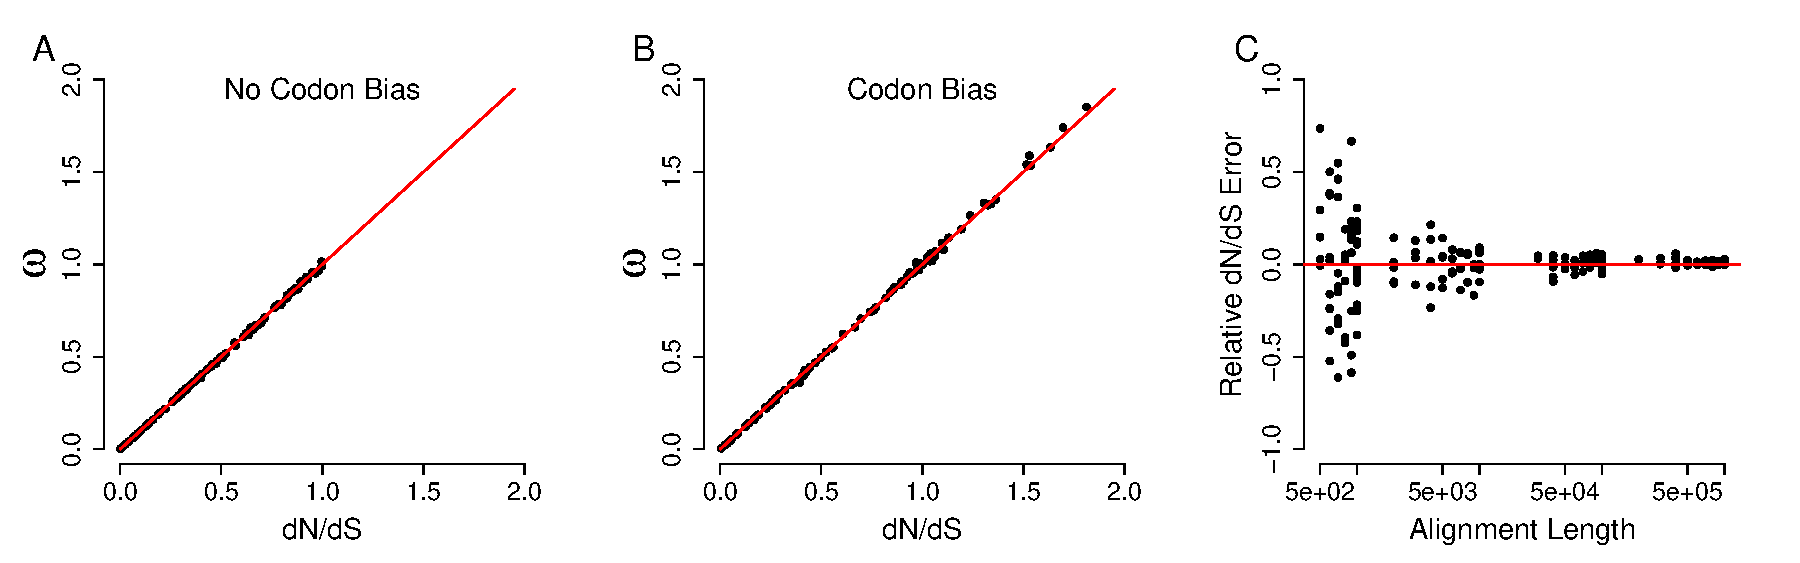
\includegraphics[width=6in]{figures/MainText/regression_convergence.pdf}}
\caption{\label{reg_conv} Relationship works exceedingly well. Left panel shows 100 points, each of which corresponds to single simulation. Note that here the ml inference is shown for equal codon frequency specs and kappa fixed to true value (a similar plot for free kappa is shown in suppfigs, but results are qualitatively identical.) Right panels shows convergence of omega values as data set size (represented as simulated alignment length) increases. The y-axis indicates relative error of the ML $dN/dS$ estimates, and the x-axis indicates sequence length on a log-scale. As the sequence length, or the data set size, increases, the two $dN/dS$ estimates converge to the same value. }
\end{figure*}


\bigskip
\begin{figure*}[H]
\centerline{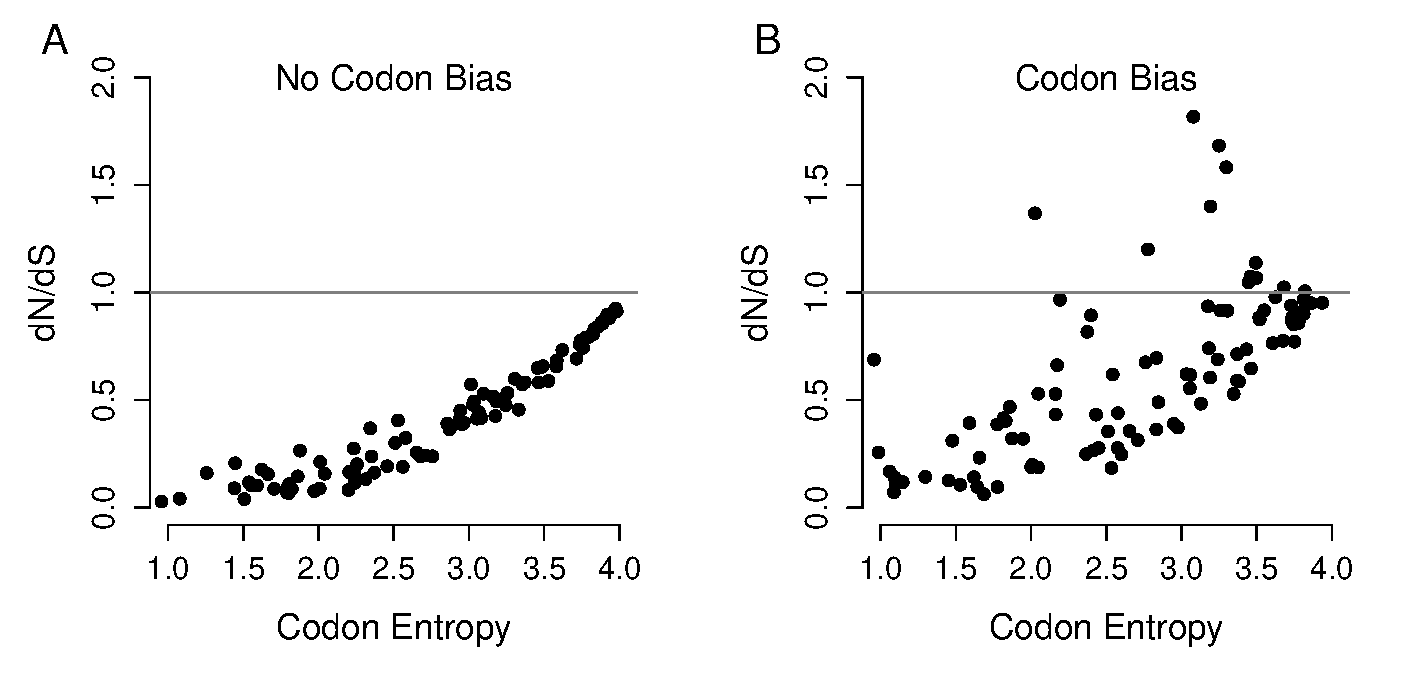
\includegraphics[width=4in]{figures/MainText/entropy_vs_dnds.pdf}}
\caption{\label{entropy_dnds} codon frequency entropy scales well with dnds but the strength of the relationship diminishes with codon bias as synonymous now have frequency differences, so dnds is less of a reliable indicator of selection strength.}
\end{figure*}


\bigskip
\begin{figure*}[H]
\centerline{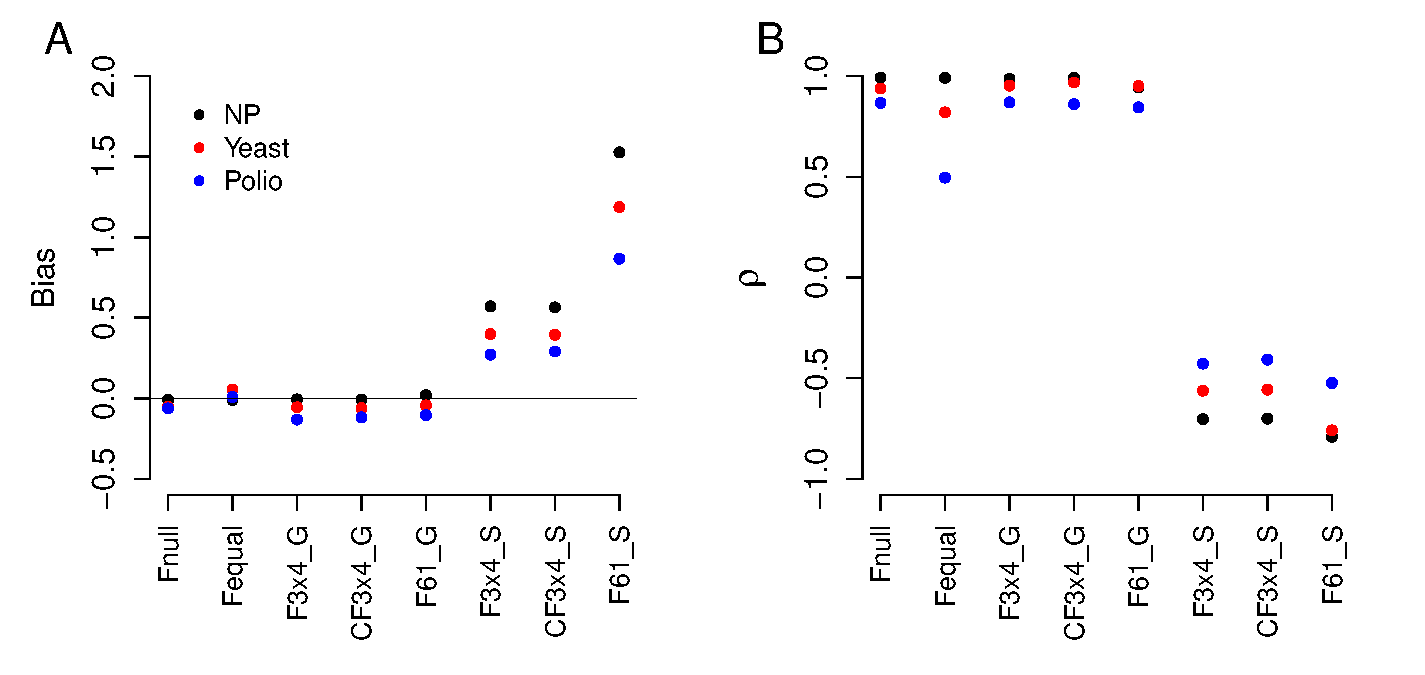
\includegraphics[width=6in]{figures/MainText/nyp_bias_corr.pdf}}
\caption{\label{nyp_bias_r2} Global outperform, obviously. Clear that the null is probably the best bet. The question is, how well to commonly used estimators approximate this null specification? Decently, but clearly F3x4 and CF3x4 do better than F61. Also, Fequal does reasonably well, but it gets noisy as the asymmetry in mutation rates grows. Site-wise sucks, and we have a good explanation for it - a lot of selection information is in there!! Bad news.}
\end{figure*}


\bigskip
\begin{figure*}[H]
\centerline{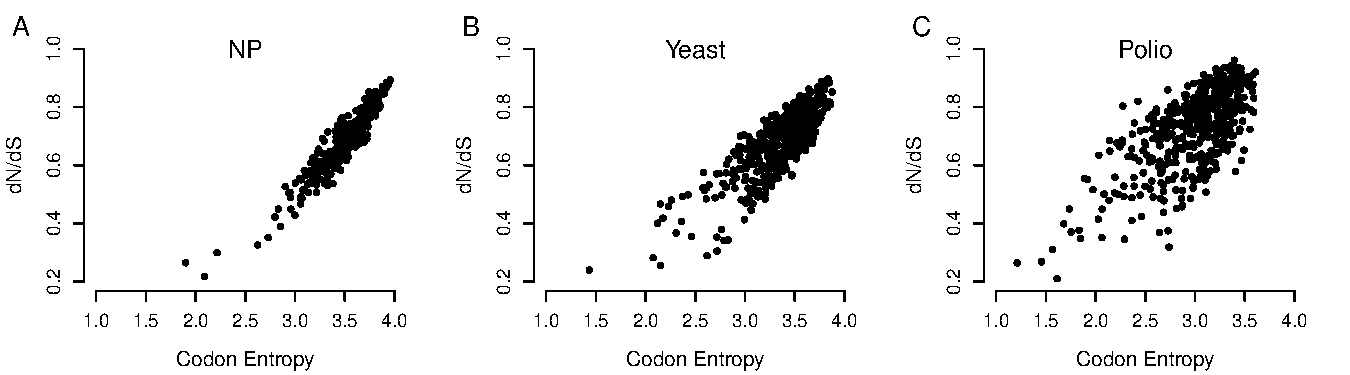
\includegraphics[width=6in]{figures/MainText/nyp_entropy_vs_dnds.pdf}}
\caption{\label{nyp_entropy_dnds} This is nice because it shows that entropy and dnds still scale really wonderfully, and noise ups as you get more asymmetric. This is because non-selection processes end up contributing to codon frequencies.}
\end{figure*}



\clearpage
\newpage

\section*{Supplementary Figures and Tables}

\begin{table}[htbp]
\customlabel{tab:tabS1}{tabS1}
\begin{tabular}{c c c c c c}
\hline\noalign{\smallskip}
\multicolumn{1}{l}{Codon frequencies} & \multicolumn{1}{l}{$\kappa$ parameterization} & \multicolumn{1}{l}{$dN/dS$ correlation} &\multicolumn{1}{l}{$dN/dS$ error} & \multicolumn{1}{l}{$\kappa$ correlation} &\multicolumn{1}{l}{$\kappa$ error} \\
\noalign{\smallskip}\hline\noalign{\smallskip}
Fequal & True & 1 & 0.02 &   &   \\ 
Fequal & Free & 0.971 & 0.105 & 0.699 & 0.262 \\ 
Fequal & 1 & 0.974 & 0.263 &   &   \\ 
\hline\noalign{\smallskip}
F3x4 & True & 0.646 & 2.134 &   &   \\ 
F3x4 & Free & 0.552 & 2.342 & 0.212 & 0.774 \\ 
F3x4 & 1 & 0.597 & 1.847 &   &   \\ 
\hline\noalign{\smallskip}
CF3x4 & True & 0.642 & 2.105 &   &   \\ 
CF3x4 & Free & 0.553 & 2.316 & 0.212 & 0.765 \\ 
CF3x4 & 1 & 0.581 & 1.845 &   &   \\ 
\hline\noalign{\smallskip}
F61 & True & -0.591 & 19.067 &   &   \\ 
F61 & Free & -0.281 & 27.714 & 0.315 & 0.927 \\ 
F61 & 1 & -0.56 & 12.272 &   &   \\ 
\noalign{\smallskip}\hline\noalign{\smallskip}
\end{tabular}
\newline
Results from runs with codon bias. Codon frequency specifications were either set as equal (1/61 per codon), calculated from the F3x4 estimator \cite{MuseGaut1994}, calculated from the CF3x4 estimator \cite{Pond2010}, or set equal to the simulated alignment's empirical frequencies. $\kappa$ was specified as either a fixed value, its true simulated value or 1, or as a free parameter of the model. Correlations given are between the ML $\omega$ estimate and our derived $\omega$ values. Error refers to the mean absolute error between these two $\omega$ estimates. Similar values for $\kappa$ are shown for those inferences where $\kappa$ was a free parameter of the model. Note that all is significant.
\end{table}	

\clearpage
\newpage

\centerline{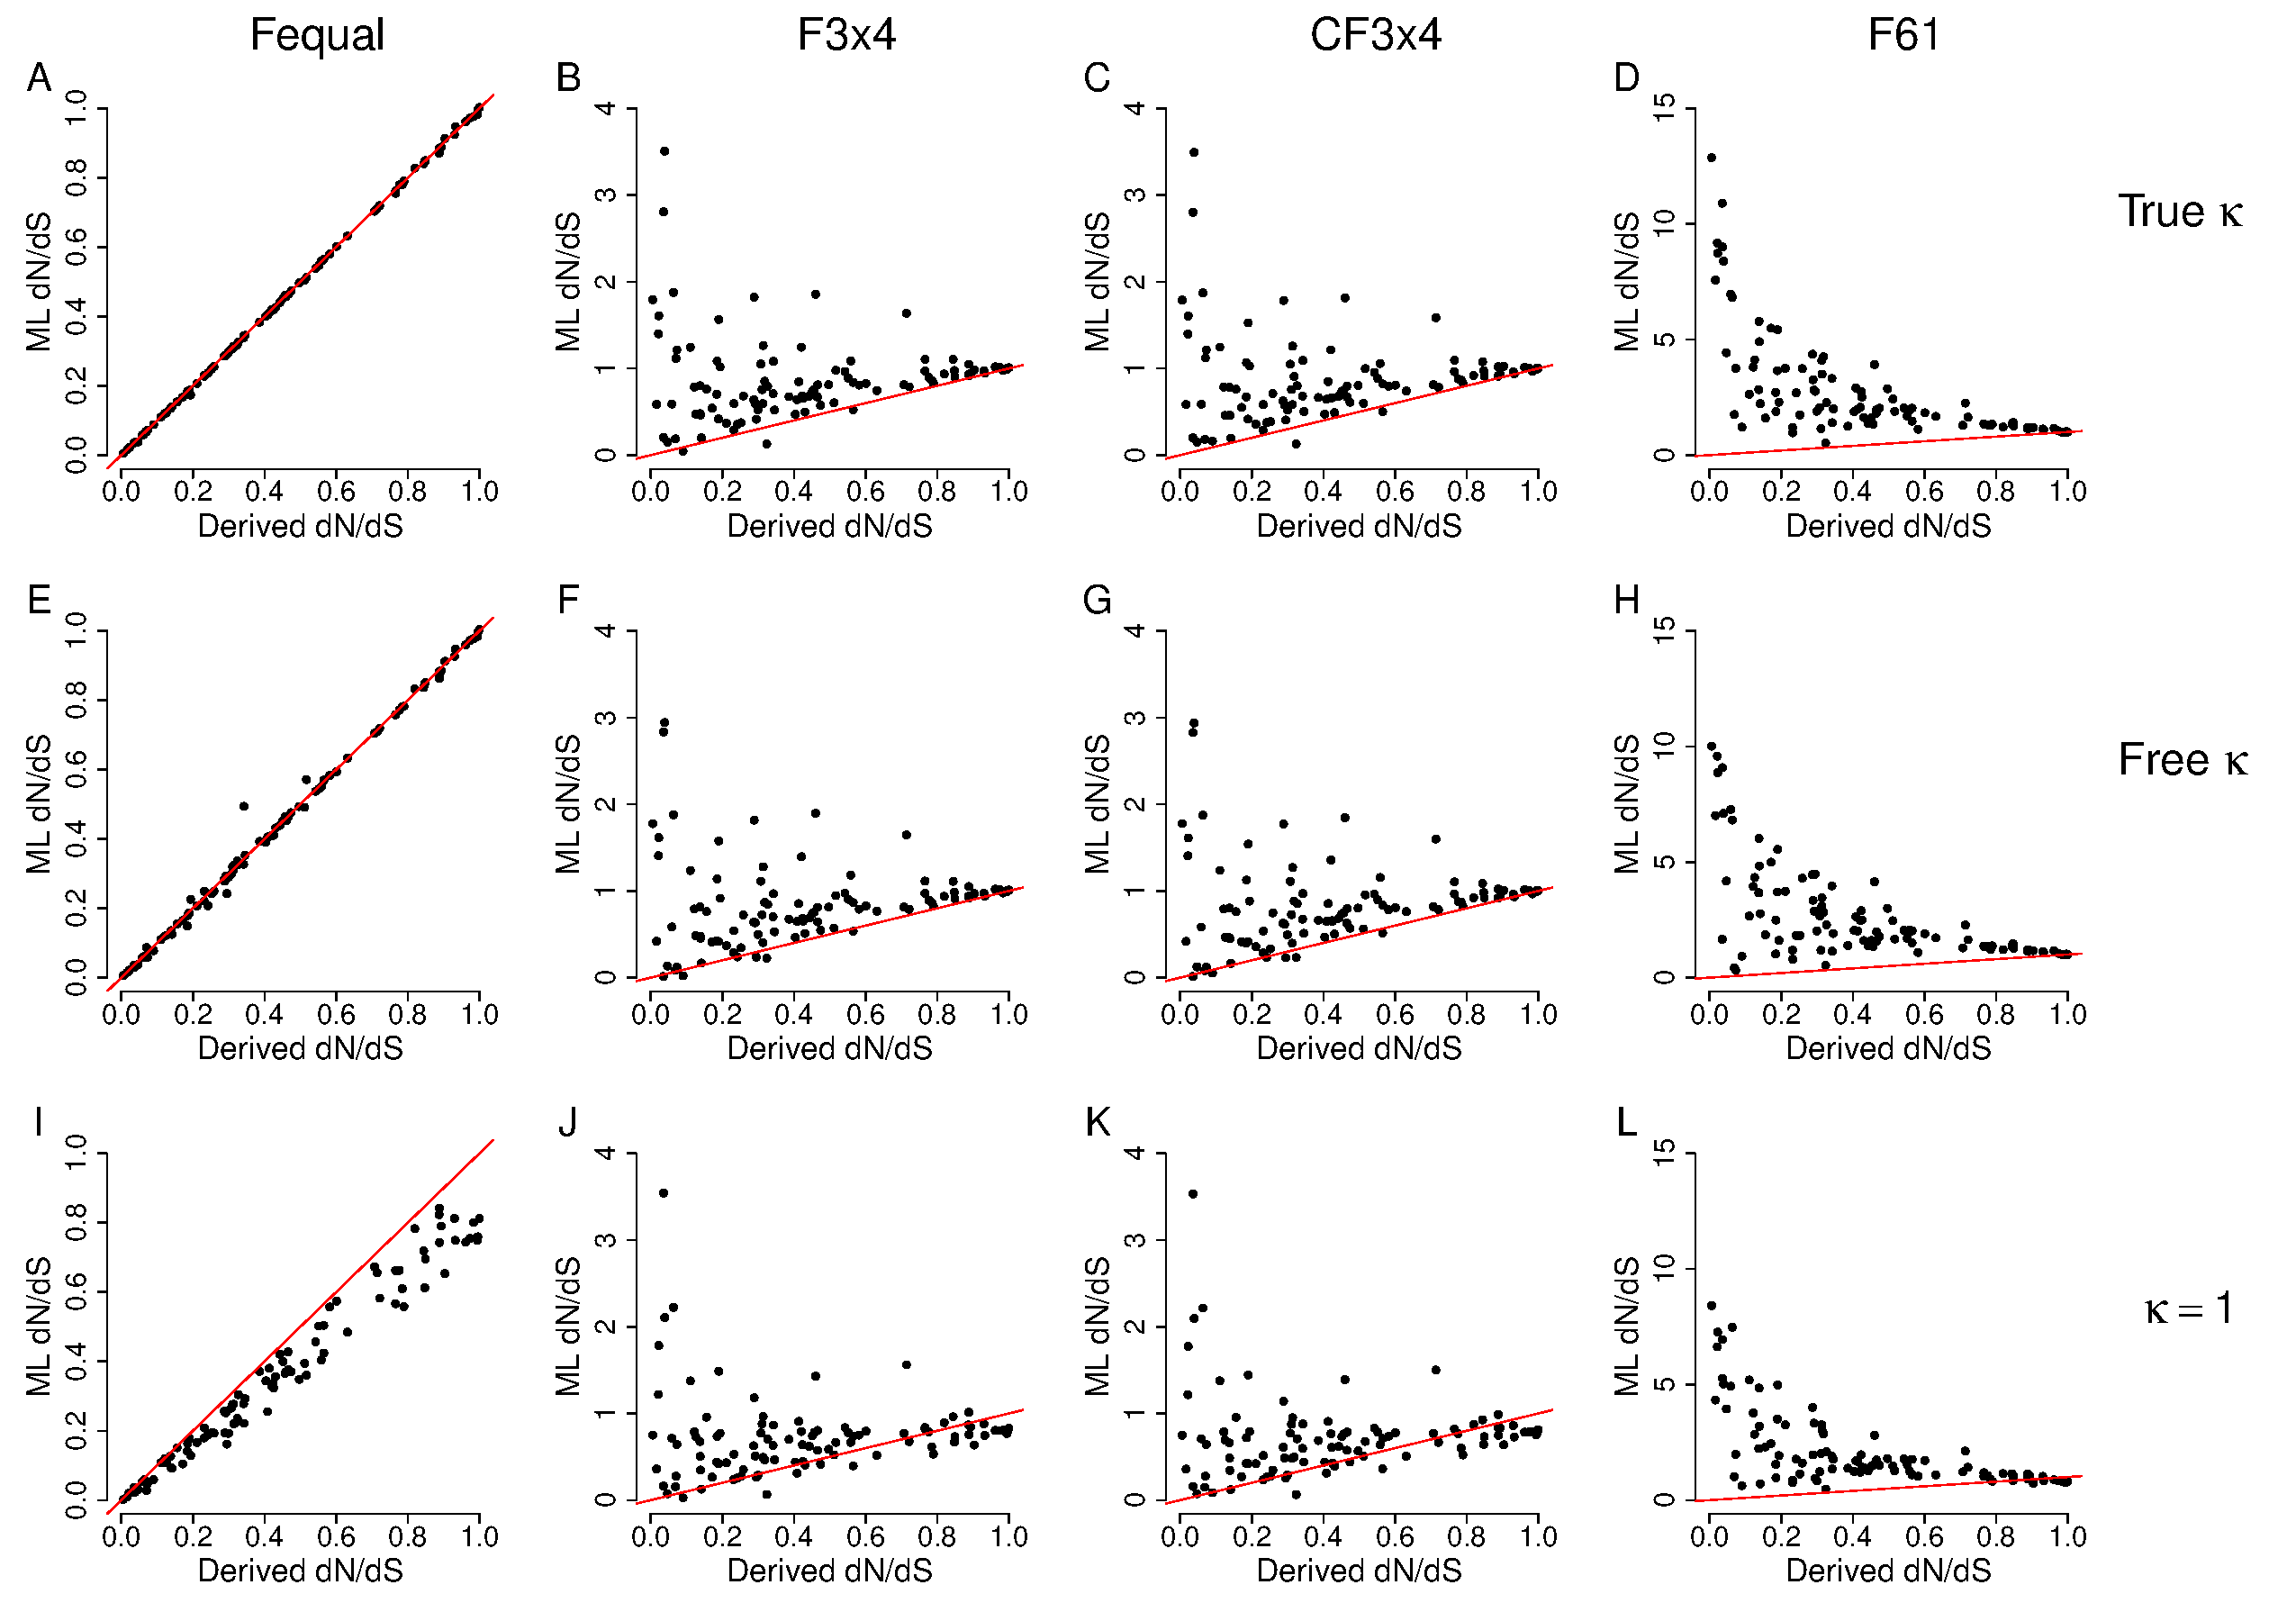
\includegraphics[width=8in]{figures/SI/regression_omega_nobias.pdf}}
\noindent \textbf{Fig. S1} Omega regression for all ML parameterizations, without codon bias.
\customlabel{fig:reg_allspecs_nobias}{S1}

\clearpage
\newpage

\centerline{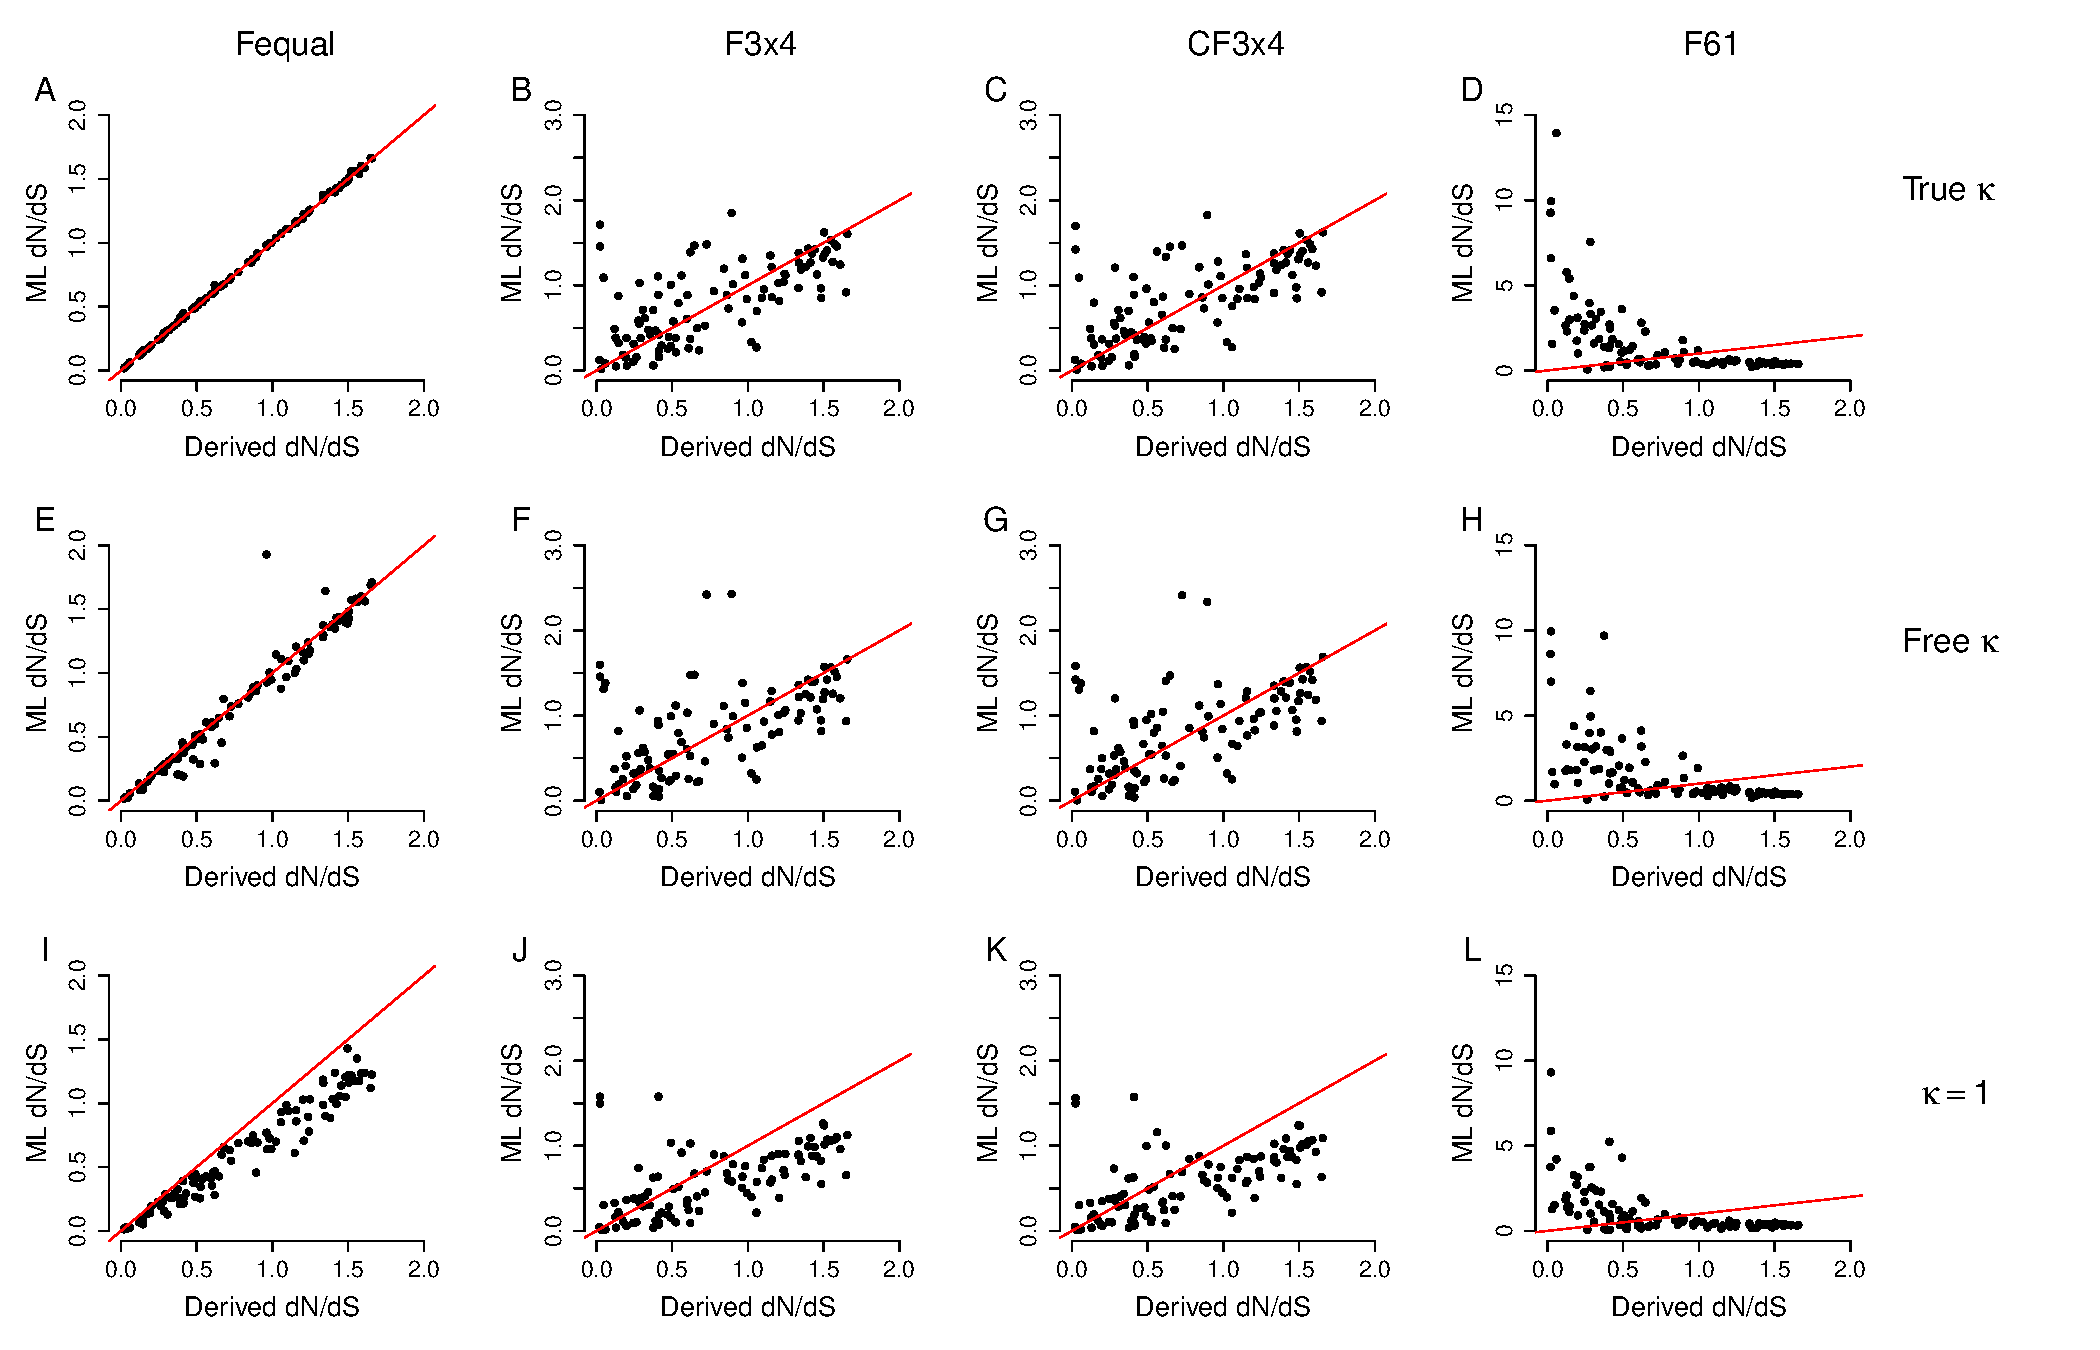
\includegraphics[width=8in]{figures/SI/regression_omega_bias.pdf}}
\noindent \textbf{Fig. S2} Omega regression for all ML parameterizations, with codon bias.
\customlabel{fig:reg_allspecs_bias}{S2}

\bigskip
\bigskip
\bigskip


\centerline{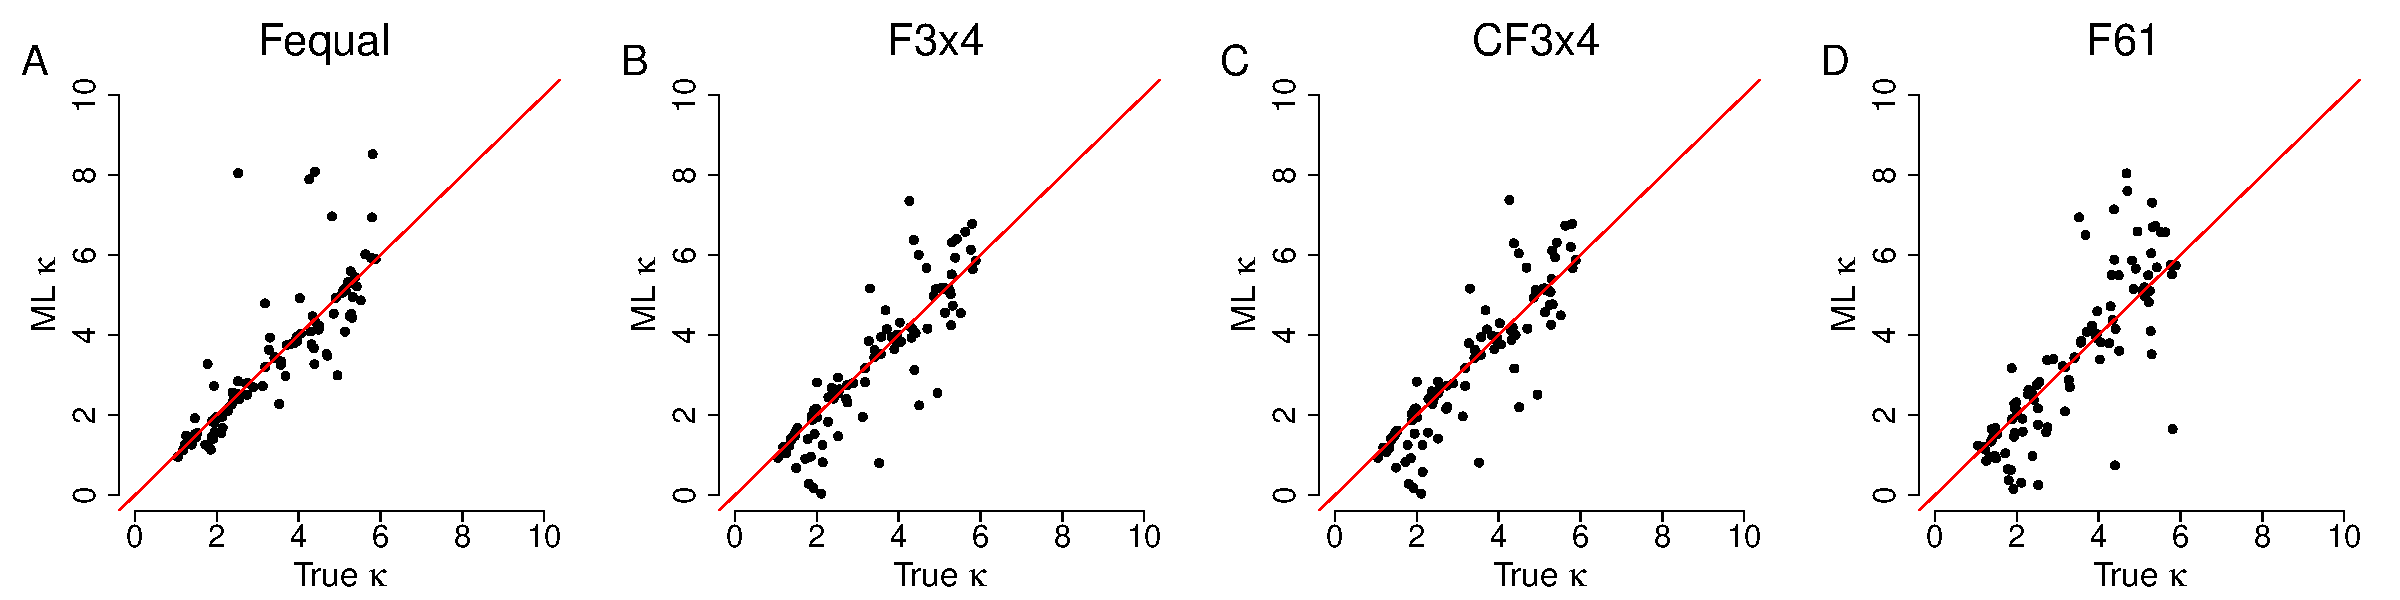
\includegraphics[width=6in]{figures/SI/regression_kappa_nobias.pdf}}
\noindent \textbf{Fig. S3} Kappa regression for all ML freqspec parameterizations where kappa is a free parameter, without codon bias.
\customlabel{fig:reg_kappa_nobias}{S3}

\bigskip
\bigskip
\bigskip


\centerline{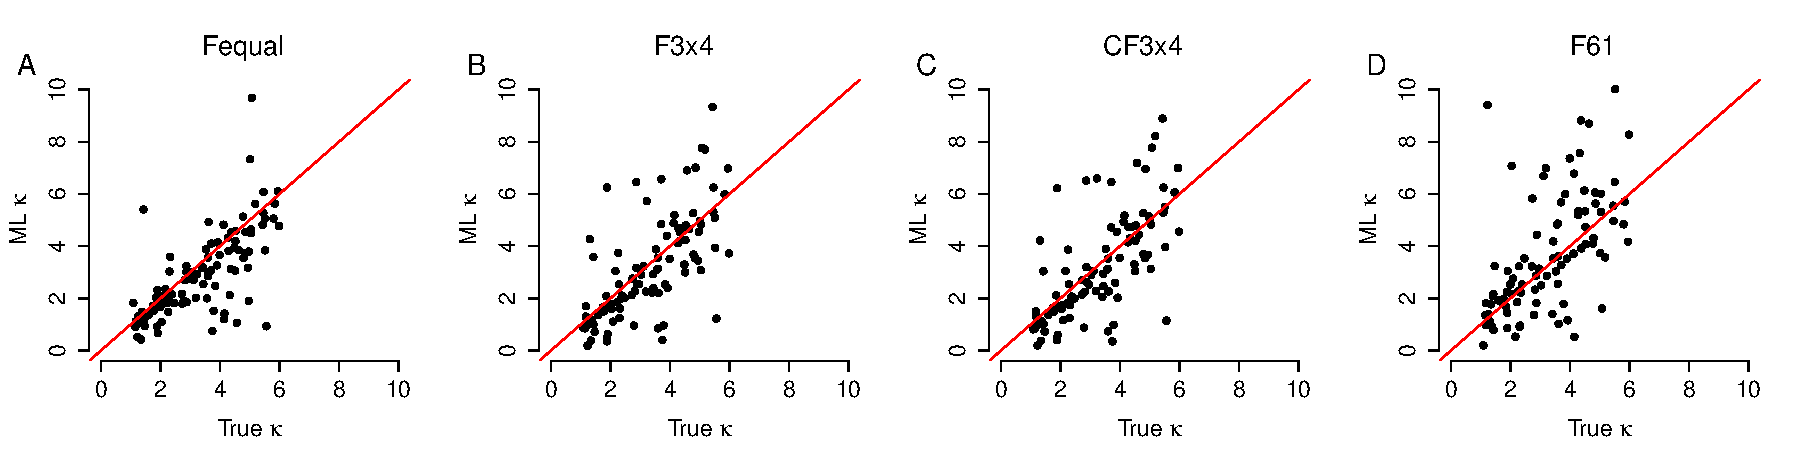
\includegraphics[width=6in]{figures/SI/regression_kappa_bias.pdf}}
\noindent \textbf{Fig. S4} Kappa regression for all ML freqspec parameterizations where kappa is a free parameter, without codon bias.
\customlabel{fig:reg_kappa_bias}{S4}


\end{document}

